% As-built Fiber-Spike-Rotor sequence mixer internals. Standalone: pdflatex this file.
\documentclass[tikz,border=8pt]{standalone}
\usepackage{amsmath,amssymb}
\usetikzlibrary{arrows.meta,positioning,fit,backgrounds,calc}
\begin{document}
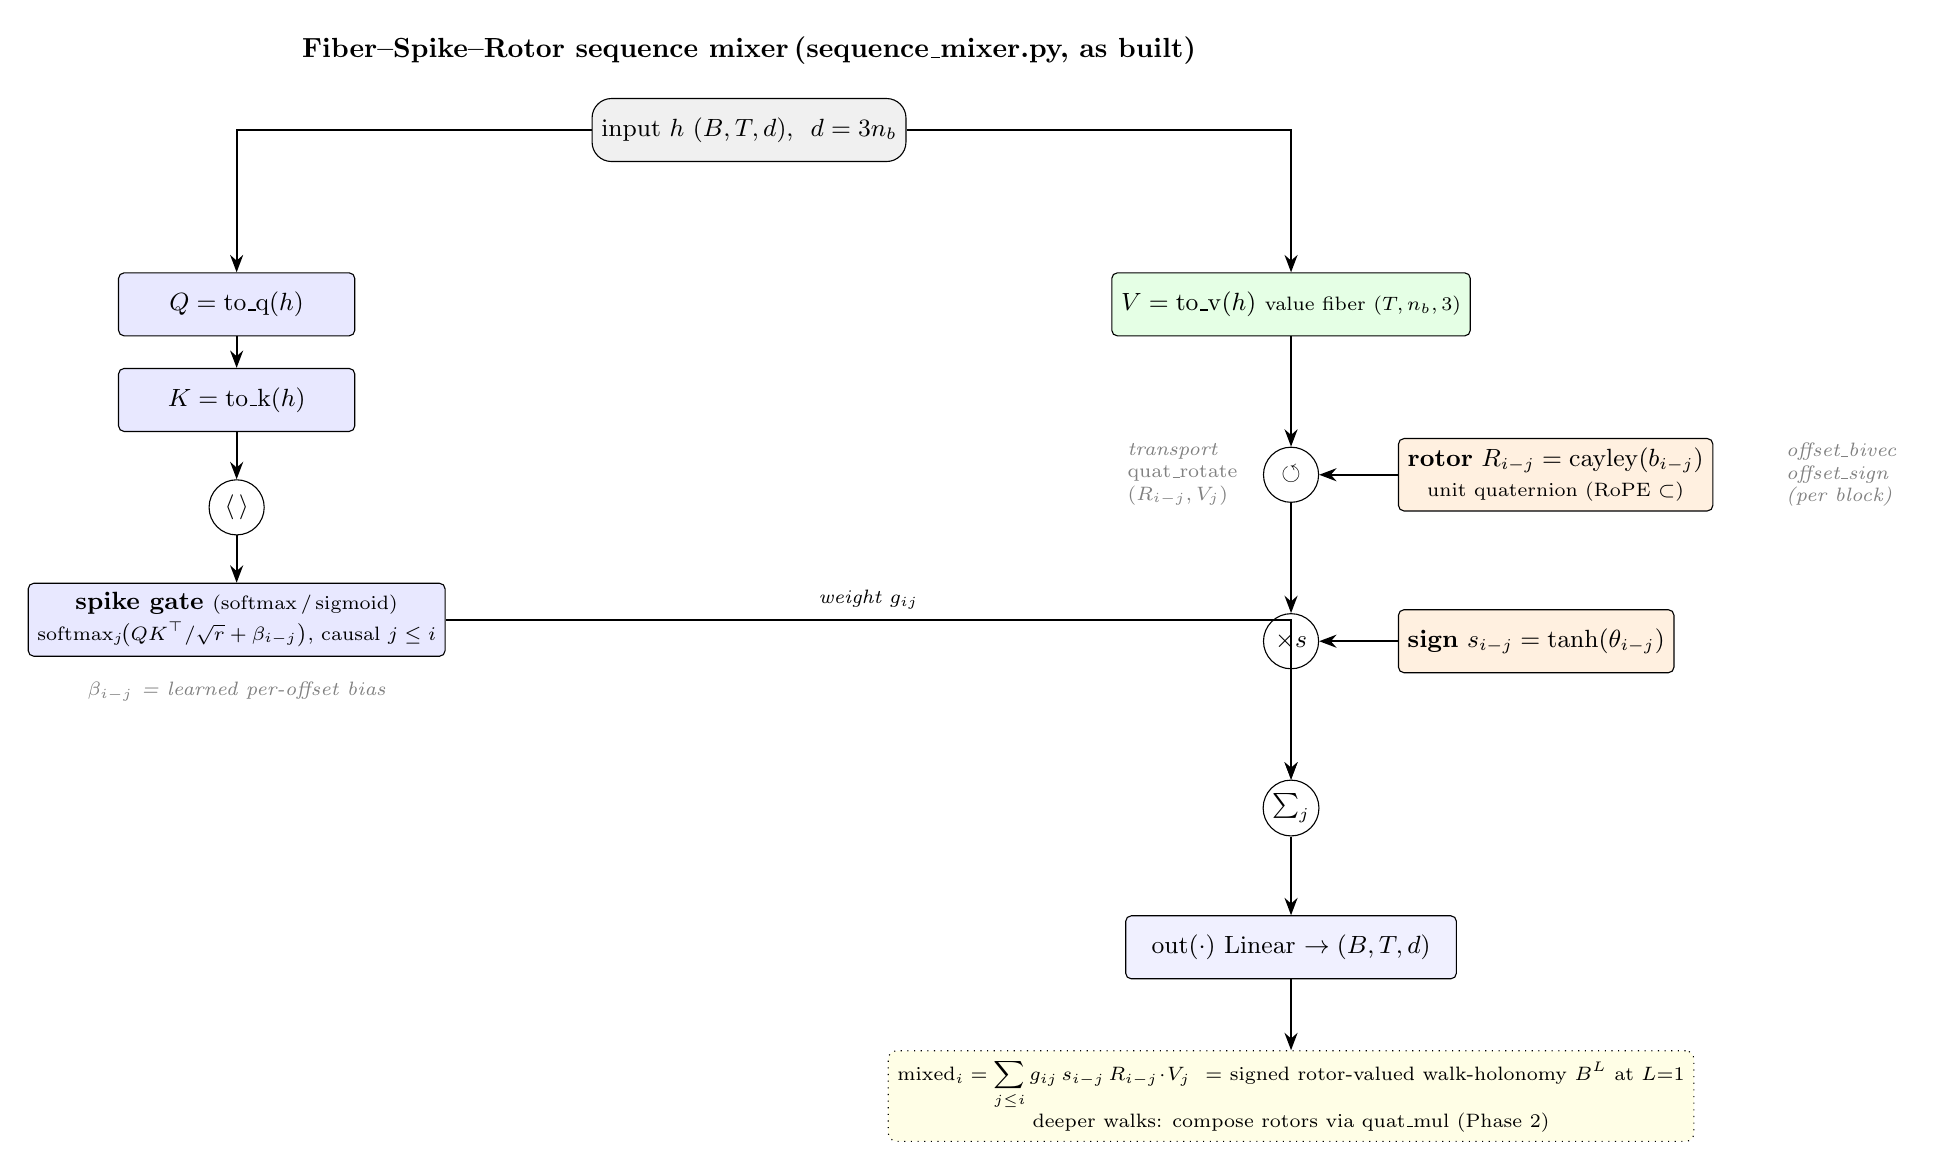
\begin{tikzpicture}[
  font=\small,>={Stealth[length=2.2mm]},
  h/.style={draw,rounded corners=7pt,fill=gray!12,align=center,minimum height=8mm},
  qk/.style={draw,rounded corners=2pt,fill=blue!9,align=center,minimum height=8mm,minimum width=30mm},
  vv/.style={draw,rounded corners=2pt,fill=green!10,align=center,minimum height=8mm,minimum width=34mm},
  rot/.style={draw,rounded corners=2pt,fill=orange!12,align=center,minimum height=8mm,minimum width=34mm},
  op/.style={draw,circle,inner sep=1pt,minimum size=7mm,fill=white},
  ar/.style={->,thick},
  note/.style={font=\scriptsize\itshape,gray,align=left}
]
\node[h] (h) {input $h\ (B,T,d)$,\ \ $d=3n_b$};

% ---- gate (spike) path : left column ----
\node[qk,below left=14mm and 30mm of h] (q) {$Q=\mathrm{to\_q}(h)$};
\node[qk,below=4mm of q] (k) {$K=\mathrm{to\_k}(h)$};
\node[op,below=6mm of k] (score) {$\langle\,\rangle$};
\node[qk,below=6mm of score,align=center,minimum width=40mm] (gate)
  {\textbf{spike gate}\ \scriptsize (softmax\,/\,sigmoid)\\ \scriptsize $\mathrm{softmax}_j\!\big(QK^\top/\sqrt r+\beta_{i-j}\big)$,\ causal $j\le i$};
\node[note,below=2mm of gate] {$\beta_{i-j}$ = learned per-offset bias};

% ---- value + connection path : right column ----
\node[vv,below right=14mm and 26mm of h] (v) {$V=\mathrm{to\_v}(h)$\ \scriptsize value fiber $(T,n_b,3)$};
\node[op,below=14mm of v] (rotate) {$\circlearrowleft$};
\node[rot,right=10mm of rotate] (rot) {\textbf{rotor} $R_{i-j}=\mathrm{cayley}(b_{i-j})$\\ \scriptsize unit quaternion\ (RoPE $\subset$)};
\node[note,left=2mm of rotate] {transport\\ $\mathrm{quat\_rotate}$\\ $(R_{i-j},V_j)$};
\node[op,below=14mm of rotate] (signmul) {$\times s$};
\node[rot,right=10mm of signmul] (sgn) {\textbf{sign} $s_{i-j}=\tanh(\theta_{i-j})$};

% ---- aggregate ----
\node[op,below=14mm of signmul] (agg) {$\sum_j$};
\node[draw,rounded corners=2pt,fill=blue!6,below=10mm of agg,align=center,minimum height=8mm,minimum width=42mm] (out)
  {$\mathrm{out}(\cdot)$ Linear $\to (B,T,d)$};
\node[note,right=8mm of rot,align=left] {offset\_bivec\\ offset\_sign\\ (per block)};

% wires
\draw[ar] (h.west) -| (q.north);
\draw[ar] (q) -- (k); \draw[ar] (k) -- (score); \draw[ar] (score) -- (gate);
\draw[ar] (h.east) -| (v.north);
\draw[ar] (v) -- (rotate);
\draw[ar] (rot) -- (rotate);
\draw[ar] (rotate) -- (signmul);
\draw[ar] (sgn) -- (signmul);
\draw[ar] (signmul) -- (agg);
\draw[ar] (gate.east) -| (agg) node[pos=0.25,above,note,black]{weight $g_{ij}$};
\draw[ar] (agg) -- (out);

% holonomy annotation
\node[draw,dotted,rounded corners=3pt,fill=yellow!10,below=9mm of out,align=center,font=\scriptsize] (holo)
 {$\displaystyle \text{mixed}_i=\sum_{j\le i} g_{ij}\,s_{i-j}\,R_{i-j}\!\cdot\!V_j$
   \ $=$ signed rotor-valued walk-holonomy $B^{L}$ at $L{=}1$\\
   deeper walks: compose rotors via quat\_mul (Phase 2)};
\draw[ar] (out) -- (holo);

\node[font=\bfseries,above=3mm of h] {Fiber--Spike--Rotor sequence mixer\,(sequence\_mixer.py, as built)};
\end{tikzpicture}
\end{document}
